\documentclass[tikz]{standalone}

\usepackage{tikz}
\usetikzlibrary{trees}
\usetikzlibrary{shapes}
\usetikzlibrary{positioning}
\usetikzlibrary{arrows.meta}

\tikzset{
    pointer/.style = {thick,draw=black,triangle 45-*,shorten >=-3pt},
    cell/.style = {rectangle, thick, draw=black,minimum width = 1cm, minimum height =1.0cm,fill=yellow!20},
    mynode/.style = {circle, thick, draw=black, align=center,fill=yellow!40,font=\ttfamily\bfseries\Large},
    mynoder/.style = {circle, thick, draw=black, align=center,fill=red!30,font=\ttfamily\bfseries\Large},
    mynodeb/.style = {circle, thick, draw=black, align=center,fill=blue!30,font=\ttfamily\bfseries\Large},
    edgen/.style = {-latex,ultra thick},
    edger/.style = {-latex,ultra thick,red},
    edgeb/.style = {-latex,ultra thick,blue},
    edgeg/.style = {-latex,ultra thick,gray},
    edgegd/.style = {-latex,ultra thick,brown,dashed}, % back
    edgevd/.style = {-latex,ultra thick,violet,dotted}, % forward
    edgexd/.style = {-latex,ultra thick,blue,densely dotted}, % traversal
    every picture/.style={/utils/exec={\ttfamily\bfseries}},
    every picture/.style={font issue=\ttfamily\bfseries},
    font issue/.style={execute at begin picture={#1\selectfont}
  }
}

\begin{document}


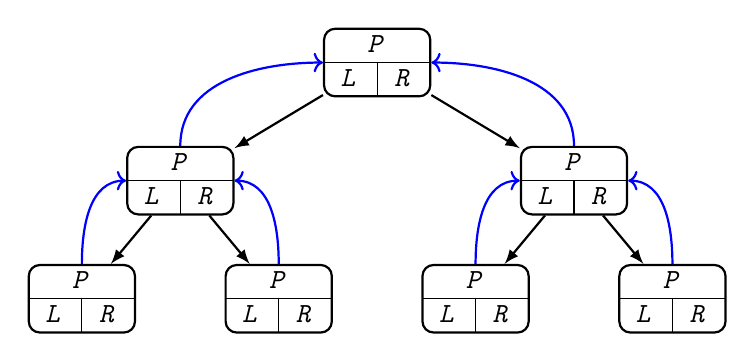
\begin{tikzpicture}[
	level distance=1.5cm,
    level 1/.style={sibling distance=5cm},
    level 2/.style={sibling distance=2.5cm},
	edge from parent/.style={draw,-latex},
	thick
]
\node[rounded corners, draw, inner sep=+0pt] (T){%
  \begin{tabular}{c|c}
    \multicolumn{2}{c}{\emph{P}} \\\hline
    \emph{L} & \emph{R}
  \end{tabular}}
	child { node[rounded corners, draw, inner sep=+0pt] (TL){%
  \begin{tabular}{c|c}
    \multicolumn{2}{c}{\emph{P}} \\\hline
    \emph{L} & \emph{R}
  \end{tabular}}
		child { node[rounded corners, draw, inner sep=+0pt] (TLL){%
	  \begin{tabular}{c|c}
	    \multicolumn{2}{c}{\emph{P}} \\\hline
	    \emph{L} & \emph{R}
	  \end{tabular}}
		}
		child { node[rounded corners, draw, inner sep=+0pt] (TLR){%
	  \begin{tabular}{c|c}
	    \multicolumn{2}{c}{\emph{P}} \\\hline
	    \emph{L} & \emph{R}
	  \end{tabular}}
		}
	}
	child {node[rounded corners, draw, inner sep=+0pt] (TR) {%
	  \begin{tabular}{c|c}
	    \multicolumn{2}{c}{\emph{P}} \\\hline
	    \emph{L} & \emph{R}
	  \end{tabular}}
		child { node[rounded corners, draw, inner sep=+0pt] (TRL){%
	  \begin{tabular}{c|c}
	    \multicolumn{2}{c}{\emph{P}} \\\hline
	    \emph{L} & \emph{R}
	  \end{tabular}}
		}
		child { node[rounded corners, draw, inner sep=+0pt] (TRR){%
	  \begin{tabular}{c|c}
	    \multicolumn{2}{c}{\emph{P}} \\\hline
	    \emph{L} & \emph{R}
	  \end{tabular}}
		}
  };
\draw[->,blue] (TL) to[out=90,in=180] (T);
\draw[->,blue] (TR) to[out=90,in=0] (T);
\draw[->,blue] (TRL) to[out=90,in=180] (TR);
\draw[->,blue] (TRR) to[out=90,in=0] (TR);
\draw[->,blue] (TLL) to[out=90,in=180] (TL);
\draw[->,blue] (TLR) to[out=90,in=0] (TL);
\end{tikzpicture}


\end{document}